\chapter{Project proposal}

\begin{center}
{\Large DRAFT Honours Project Proposal:
Capacity Control in Boosting via an Adjustable  b Function
\footnote{This project was originally called, ``Aspects
of Statistical Learning Theory and Support Vector Machines''} \\
Jeremy Barnes \\
Supervisor: Dr Bob Williamson}
\end{center}

\section{Introduction}
The aim of this document is to provide some detail on the scope and
implementation of this honours project.  A brief background on the
project is given; followed by an explicit statement of the expected
outcomes; and a timeline.

\section{Background}
Boosting is a method used to improve the generalisation ability of a
"weak" learning algorithm.  It is implemented by generating many
instances of the algorithm, each trained on different data.  This data
is chosen such that examples which are commonly misclassified are
emphasised.  This forces the learning algorithm to work well with the
difficult data, and have better overall performance.  The output of
the boosting algorithm is a weighted combination of the outputs of the
weak learning algorithms (weighted by their performance).

Adjusting the capacity of a learning algorithm controls the size of
the set of possible generalisations.  It is important to control
capacity to avoid overfitting (fitting the noise rather than the
underlying function).  Although boosting is particularly good at
avoiding overfitting, implementing capacity control can improve the
performance of the boosted algorithm [ref] and avoid eventual
overfitting.

The $b$ function is used within the boosting algorithm.  It is
calculated for each instance of the weak learning algorithm, from the
learning error of the weak learning algorithm (the learning error is
the proportion of samples which are misclassified).  In the case of a
binary classification problem, it has the form
%
\begin{equation}
b_t = \log \frac{\epsilon_t}{1-\epsilon_t} \qquad (0 \leq \epsilon_t
\leq 1)
\end{equation}
%	
where $\epsilon_t$ is the learning error of weak learning algorithm  $t$.

	This function describes the ``worth'' of this instance of the weak
learning algorithm.  A plot is shown in figure 1.

\begin{figure}
\begin{center}
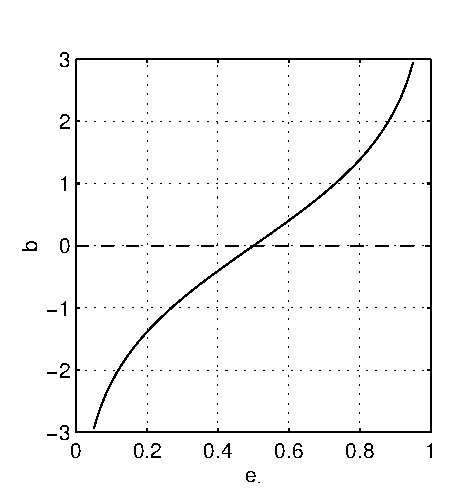
\includegraphics{figures/bfunc.epsg}
\end{center}
\caption{The $b_t$ function versus error $\epsilon_t$}
\end{figure}
 
Weak learners with a value of $\epsilon_t$ around $1/2$ are worthless,
as random guessing performs just as well.  As $epsilon_t$ moves away
from $1/2$, the algorithms become more useful (and show an increase in
$b_t$ ).  Algorithms that approach $\epsilon_t \rightarrow \pm 1$ are
given a $b_t$  that approaches $\pm \infty$.

This project will investigate modifying the b function to become
\begin{equation}
b^{\prime}_t = \mathrm{sign}(b_t) |b_t|^{1/p}
\end{equation}
The new parameter p allows control over how aggressively weak learners
are penalised.  This should allow capacity control via adjustment of
this parameter.

\section{Outcomes}
The project will be successful if the following outcomes are attained:

\begin{itemize}
\item	Enough experimental evidence is gathered to gain an
	appreciation of the effect of the   parameter on the boosting
	algorithm.

\item	From this evidence, some guiding principles for improving the
	performance of the boosting algo-rithm using the   parameter
	are developed.

\item	Theoretical justification of these results is obtained.
\end{itemize}

In addition to these goals, it is hoped that progress in one or more of the following areas will be made:

\begin{itemize}
\item	Performance of the algorithm in problems with varying amounts
	of noise;

\item	Improved versions on the p-boosting algorithm using knowledge
	gained from the theory;

\item	Improving the computational efficiency of boosting using the
	p-boosting algorithm;

\item	Comparisons between p-boosting and other methods of capacity
	control in boosting;

\item	Extension of the results to include arbitrary classification
	problems;

\item	Extension of the results to include regression problems;

\item	Extension of the results to include other enhancements to the
	boosting algorithm, such as "soft margins" \cite{Ratsch98}.
\end{itemize}

In order to limit the project to a reasonable scope, initially the following constraints will be placed:

\begin{itemize}
\item	Only binary classification problems will be considered.

\item	Small datasets will be used.

\item	Simple weak learning algorithms will be used.
\end{itemize}


\section{Timeline}
This section includes a month-by-month description of what I intend to
complete on the project.  It is given in table \ref{table:timeline} on
page \pageref{table:timeline}.

\begin{table}
\begin{tabular}{r l}
\textbf{Month}		& \textbf{Tasks} \\ \hline \hline
December 1998		& Reading \\ \hline
January 1999		& Reading \\ \hline
February 		& Reading \\ \hline
March			& Writing project proposal \\
			& \textbf{19th Project proposal due} \\
			& Obtaining or writing code for experiments \\ \hline
April			& Writing, debugging code \\
			& 12th Code running, first test results \\
			& Obtaining datasets, running tests, refining
			  code  \\ \hline
May			& Running tests \\
			& Developing and testing hypotheses \\
			& Reading on theory \\
			& \textbf{31st First draft of "background"
			  section of thesis} \\ \hline
June			& Initial attempts at theoretical analysis \\
			& Running tests required for theoretical
			  verification \\
			& Attempting to reach closure on some aspects \\
			& \textbf{Exam period} \\ \hline
July			& Attempting to reach closure on some aspects \\
			& Writing progress report \\
			& \textbf{19th Progress report due} \\
			& Preparing for seminar \\
			& \textbf{26th Seminar} \\ \hline
August			& Final work on theory \\
			& Final experimental results to assist theory \\
			& \textbf{30th Sufficient work done to
			  complete thesis} \\ \hline
September		& Work on spin-off or extension aspects \\
			& Preparing for demonstration \\
			& \textbf{27th All experimental and
			  theoretical results obtained} \\
			& Writing thesis \\ \hline
October			& Writing thesis \\
			& \textbf{7th Draft thesis due} \\
			& Revising thesis \\
			& \textbf{27th Thesis due} \\
			& \textbf{28th Demonstration} \\
\hline
\end{tabular}
\caption{Project timeline}
\label{table:timeline}
\end{table}

\noindent\textbf{Notes:}

\begin{itemize}
\item 	I intend to work on the thesis gradually throughout the year,
	so that I do not need to write it all at the end.

\item	I have allowed 2-3 weeks to work on "extension" aspects of the
	problem that are interesting but not vital to a strong thesis.  It
	would not be a serious problem if none of this work can be included in
	the thesis.  These 2-3 weeks also give me some slack if things are not
	going as planned or if I become burnt out and need a break.
\end{itemize}

